\documentclass[aspectratio=169, table]{beamer}
\usetheme{Madrid}
\usecolortheme{default}

% --- REPLACE/UPDATE PREAMBLE ---
\usepackage{graphicx}
\usepackage{booktabs}
\usepackage{amsmath}
\usepackage{tikz}
\usetikzlibrary{shapes,arrows,positioning,shadows.blur,calc,matrix}
\usepackage{pgfplots}
\pgfplotsset{compat=newest}
\usepackage{listings}
\usepackage{pifont}
\usepackage[most]{tcolorbox} % Modern boxes for code/alerts

% Define consistent colors
\definecolor{acadblue}{RGB}{0, 51, 102}
\definecolor{acadgreen}{RGB}{46, 139, 87}
\definecolor{acadred}{RGB}{178, 34, 34}
\definecolor{codebg}{gray}{0.95}

% Improved Code Listing Style
\tcbset{
    codestyle/.style={
        enhanced,
        colback=codebg,
        colframe=gray!20,
        boxrule=0.5pt,
        arc=2pt,
        left=2pt, right=2pt, top=2pt, bottom=2pt,
        fontupper=\tiny\ttfamily
    }
}

\title{GPU-Accelerated Track Reconstruction Optimization}
\subtitle{Multi-Event Batching for the ACTS/traccc Framework}
\author{Hao-Chun, Liang}
\institute{Master's Thesis Progress Report}
\date{January 2026}

\begin{document}

%--- Title Slide ---%
\begin{frame}
\titlepage
\vspace{-1em}
\centering{\small Advisor: Prof. Bo-Cheng, Lai}
\end{frame}

%--- Outline ---%
\begin{frame}{Outline}
\tableofcontents
\end{frame}

%==============================================================================%
\section{Project Overview}
%==============================================================================%

\begin{frame}{Project Context}
\begin{columns}
\column{0.5\textwidth}
\textbf{What is traccc?}
\begin{itemize}
    \item Track reconstruction for particle physics
    \item Part of ACTS project (CERN)
    \item GPU-accelerated using CUDA
    \item Critical for HL-LHC data processing
\end{itemize}

\vspace{0.5em}
\textbf{Focus Area}
\begin{itemize}
    \item Combinatorial Kalman Filter (CKF)
    \item Most compute-intensive component
    \item Target: High-pileup events ($\mu=200$)
\end{itemize}

\column{0.5\textwidth}
\centering
% UPDATED: Increased vertical spacing (y-coordinates spread out)
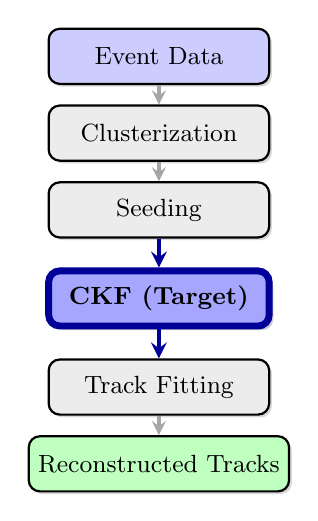
\begin{tikzpicture}[scale=0.75,
    box/.style={draw, rounded corners=4pt, minimum width=2.8cm, minimum height=0.7cm, font=\small, line width=0.8pt},
    arrow/.style={->, thick, >=stealth, line width=1.2pt}]
    
    % Spread y-coordinates: 3.2 -> 2.1 -> 1.0 -> -0.2 -> -1.4 -> -2.6
    \node[box, fill=blue!20, drop shadow={shadow xshift=1pt, shadow yshift=-1pt, opacity=0.3}] (input) at (0,3.5) {Event Data};
    \node[box, fill=gray!15, drop shadow={shadow xshift=1pt, shadow yshift=-1pt, opacity=0.3}] (cluster) at (0,2.2) {Clusterization};
    \node[box, fill=gray!15, drop shadow={shadow xshift=1pt, shadow yshift=-1pt, opacity=0.3}] (seed) at (0,0.9) {Seeding};
    \node[box, fill=blue!35, line width=2.5pt, draw=blue!60!black, drop shadow={shadow xshift=1.5pt, shadow yshift=-1.5pt, opacity=0.4}] (ckf) at (0,-0.6) {\textbf{CKF (Target)}};
    \node[box, fill=gray!15, drop shadow={shadow xshift=1pt, shadow yshift=-1pt, opacity=0.3}] (fit) at (0,-2.1) {Track Fitting};
    \node[box, fill=green!25, drop shadow={shadow xshift=1pt, shadow yshift=-1pt, opacity=0.3}] (output) at (0,-3.4) {Reconstructed Tracks};

    \draw[arrow, color=gray!70] (input) -- (cluster);
    \draw[arrow, color=gray!70] (cluster) -- (seed);
    \draw[arrow, color=blue!60!black, line width=1.5pt] (seed) -- (ckf);
    \draw[arrow, color=blue!60!black, line width=1.5pt] (ckf) -- (fit);
    \draw[arrow, color=gray!70] (fit) -- (output);
\end{tikzpicture}
\end{columns}
\end{frame}

\begin{frame}{Research Objectives}
\begin{block}{Primary Goal}
    Improve GPU throughput of the Combinatorial Kalman Filter (CKF) algorithm for high-pileup LHC events
\end{block}

\vspace{0.5em}
\textbf{Specific Objectives:}
\begin{enumerate}
    \item Implement multi-event batching to improve GPU utilization
    \item Optimize memory access patterns (constant/texture memory)
    \item Reduce synchronization overhead in CUDA kernels
    \item Validate correctness across 1,460+ test cases
\end{enumerate}

\vspace{0.5em}
\begin{alertblock}{Success Metric}
    Target: $\geq$50\% throughput improvement while maintaining physics accuracy
\end{alertblock}
\end{frame}

%==============================================================================%
\section{Methodology}
%==============================================================================%

\begin{frame}{Optimization Approach}
\begin{columns}
\column{0.5\textwidth}
% Circular Development Cycle
\centering
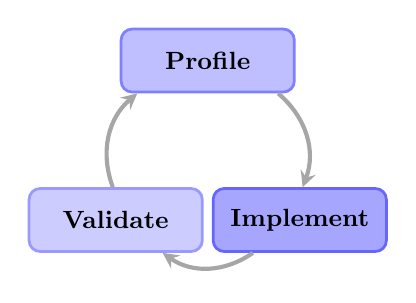
\begin{tikzpicture}[scale=0.9, >=stealth]
    \def\radius{1.5cm}
    % Nodes in a circle - unified blue color scheme
    \node[draw, rounded corners, fill=blue!25, minimum width=2.2cm, minimum height=0.8cm, line width=1pt, draw=blue!50] (profile) at (90:\radius) {\small \textbf{Profile}};
    \node[draw, rounded corners, fill=blue!35, minimum width=2.2cm, minimum height=0.8cm, line width=1pt, draw=blue!60] (implement) at (330:\radius) {\small \textbf{Implement}};
    \node[draw, rounded corners, fill=blue!20, minimum width=2.2cm, minimum height=0.8cm, line width=1pt, draw=blue!40] (validate) at (210:\radius) {\small \textbf{Validate}};
    % Curved arrows - thicker with visible arrowheads
    \draw[->, line width=1.5pt, bend left=35, color=gray!70] (profile) to (implement);
    \draw[->, line width=1.5pt, bend left=35, color=gray!70] (implement) to (validate);
    \draw[->, line width=1.5pt, bend left=35, color=gray!70] (validate) to (profile);
\end{tikzpicture}

\vspace{0.3em}
\textbf{Profiling Tools}
\begin{itemize}
    \item NVIDIA Nsight Systems (NSYS)
    \item NVIDIA Nsight Compute (NCU)
\end{itemize}

\column{0.5\textwidth}
% Big Numbers - Key Bottlenecks
\centering
\textbf{Key Bottlenecks Identified}

\vspace{0.5em}
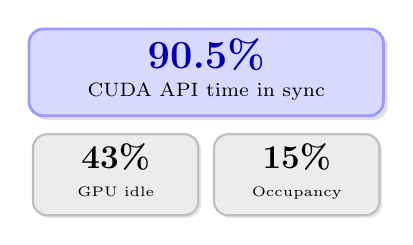
\begin{tikzpicture}
    % 90.5% box - with shadow
    \node[draw, rounded corners=5pt, fill=blue!15, minimum width=4.5cm, minimum height=1.1cm, line width=1pt, draw=blue!40, drop shadow={shadow xshift=1.5pt, shadow yshift=-1.5pt, opacity=0.25}] at (0,0) {
        \begin{tabular}{c}
            {\Large \textbf{\textcolor{blue!70!black}{90.5\%}}} \\[-2pt]
            {\scriptsize CUDA API time in sync}
        \end{tabular}
    };
    % 43% and 15% boxes side by side - with shadows
    \node[draw, rounded corners=5pt, fill=gray!15, minimum width=2.1cm, minimum height=0.9cm, line width=0.8pt, draw=gray!50, drop shadow={shadow xshift=1pt, shadow yshift=-1pt, opacity=0.2}] at (-1.15,-1.3) {
        \begin{tabular}{c}
            {\large \textbf{43\%}} \\[-2pt]
            {\tiny GPU idle}
        \end{tabular}
    };
    \node[draw, rounded corners=5pt, fill=gray!15, minimum width=2.1cm, minimum height=0.9cm, line width=0.8pt, draw=gray!50, drop shadow={shadow xshift=1pt, shadow yshift=-1pt, opacity=0.2}] at (1.15,-1.3) {
        \begin{tabular}{c}
            {\large \textbf{15\%}} \\[-2pt]
            {\tiny Occupancy}
        \end{tabular}
    };
\end{tikzpicture}

\vspace{0.3em}
{\small \textbf{Hardware:} Tesla V100 | CUDA 12.6 | ttbar\_mu200}
\end{columns}
\end{frame}

%==============================================================================%
\section{Implementation}
%==============================================================================%

\begin{frame}{Multi-Event Batching Architecture}
\begin{columns}
\column{0.45\textwidth}
\textbf{Core Innovation}
\begin{itemize}
    \item Process N events simultaneously in single CKF invocation
    \item Concatenate seeds and measurements with offset arrays
    \item Event boundary enforcement via binary search
\end{itemize}

\vspace{0.5em}
\textbf{Key Components Implemented}
\begin{itemize}
    \item \texttt{batch\_metadata} structure
    \item \texttt{get\_event\_id()} device function
    \item Device-side measurement concatenation
    \item Batched CKF wrapper ($\sim$260 lines)
\end{itemize}

\column{0.55\textwidth}
\centering
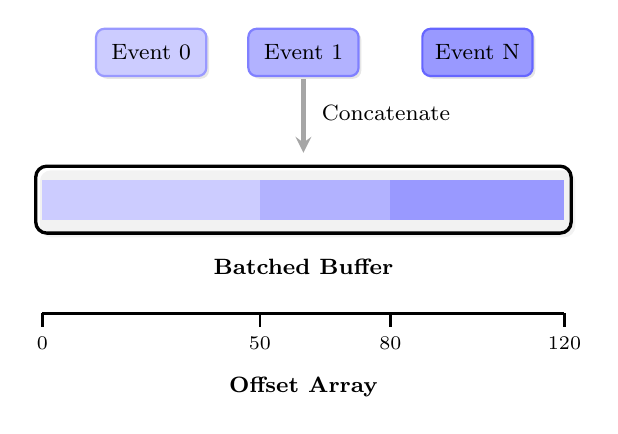
\begin{tikzpicture}[scale=0.85, >=stealth]
    % 增加比例尺 (0.04 -> 0.065)，物理上拉開 0, 50, 80, 120 的距離以解決重疊
    \def\s{0.065} 

    % --- 上方 Event 節點 (縮減寬度並配合新比例尺) ---
    % Event 0 放在 0-50 的中央 (x=25)
    \node[draw, fill=blue!20, minimum width=1.4cm, minimum height=0.6cm, 
    rounded corners=3pt, line width=0.8pt, draw=blue!40, drop shadow={shadow xshift=1pt, shadow yshift=-1pt, opacity=0.2}] 
    (e0) at ({25*\s}, 3.5) {\footnotesize Event 0};
    
    % Event 1 放在 Buffer 中央 (x=60)
    \node[draw, fill=blue!30, minimum width=1.4cm, minimum height=0.6cm, 
    rounded corners=3pt, line width=0.8pt, draw=blue!50, drop shadow={shadow xshift=1pt, shadow yshift=-1pt, opacity=0.2}] 
    (e1) at ({60*\s}, 3.5) {\footnotesize Event 1};

    % Event N 放在 80-120 的中央 (x=100)
    \node[draw, fill=blue!40, minimum width=1.4cm, minimum height=0.6cm, 
    rounded corners=3pt, line width=0.8pt, draw=blue!60, drop shadow={shadow xshift=1pt, shadow yshift=-1pt, opacity=0.2}] 
    (en) at ({100*\s}, 3.5) {\footnotesize Event N};

    % 箭頭與標籤 (垂直指向 Buffer 中央)
    \draw[->, line width=1.5pt, color=gray!70] ({60*\s}, 3.1) -- ({60*\s}, 2.0);
    \node[right, font=\footnotesize] at ({62*\s}, 2.6) {Concatenate};

    % --- Batched Buffer 外框 (維持與下方刻度 0, 120 精確對齊) ---
    \draw[line width=1.2pt, rounded corners=4pt, drop shadow={shadow xshift=1.5pt, shadow yshift=-1.5pt, opacity=0.1}] 
    (-0.1, 0.8) rectangle ({120*\s + 0.1}, 1.8);
    \node[font=\footnotesize\bfseries] at ({60*\s}, 0.3) {Batched Buffer};

    % --- 內部區塊 (0-50, 50-80, 80-120) 顏色區塊邊界與刻度線絕對對齊 ---
    \fill[blue!20] (0, 1.0) rectangle ({50*\s}, 1.6);
    \fill[blue!30] ({50*\s}, 1.0) rectangle ({80*\s}, 1.6);
    \fill[blue!40] ({80*\s}, 1.0) rectangle ({120*\s}, 1.6);

    % --- Offset Array 刻度線與標籤 ---
    \draw[line width=0.8pt] (0, -0.4) -- ({120*\s}, -0.4);
    \foreach \val in {0, 50, 80, 120} {
        \draw[line width=0.8pt] ({\val*\s}, -0.4) -- ({\val*\s}, -0.6);
        \node[font=\scriptsize, anchor=north] at ({\val*\s}, -0.6) {\val};
    }
    \node[font=\footnotesize\bfseries] at ({60*\s}, -1.5) {Offset Array};
\end{tikzpicture}
\end{columns}
\end{frame}

\begin{frame}[fragile]{Memory Optimizations}
\begin{columns}
\column{0.5\textwidth}
\textbf{1. Constant Memory for Event Offsets}
\begin{itemize}
    \item Moved offset arrays to \texttt{\_\_constant\_\_} memory
    \item Zero-latency access (vs 400 cycles global)
    \item Saves $\sim$3,200 cycles per measurement
    \item Result: \textbf{+3.7\%} (combined with texture: +6.2\%)
\end{itemize}

\vspace{1.0em}

% UPDATED: Used tcolorbox [codestyle]
\begin{tcolorbox}[codestyle, title={Constant Declaration}, top=2pt, bottom=2pt]
\begin{lstlisting}[language=C++]
__constant__ unsigned int
    c_seed_offsets[MAX_BATCH_SIZE + 1];
__constant__ unsigned int
    c_measurement_offsets[MAX_BATCH_SIZE + 1];
\end{lstlisting}
\end{tcolorbox}

\column{0.5\textwidth}
\textbf{2. Texture Memory for B-Field}
\begin{itemize}
    \item Hardware-accelerated 3D spatial lookups
    \item Enabled realistic inhomogeneous field
    \item Better cache locality for RK stepper
    \item Result: \textbf{+2.7\%}
\end{itemize}

\vspace{0.5em}
\textbf{3. Thrust::seq Replacement}
\begin{itemize}
    \item Replaced with inline device functions
    \item \texttt{inline\_lower\_bound()}
    \item \texttt{inline\_find()}, \texttt{inline\_count()}
    \item Result: \textbf{+7.8\%}
\end{itemize}
\end{columns}
\end{frame}

% --- REPLACE SLIDE 8 ---
\begin{frame}[fragile]{Synchronization Optimization}
\begin{columns}
% LEFT COLUMN: BEFORE
    \column{0.48\textwidth}
    \begin{tcolorbox}[enhanced, title={\textbf{Before (Blocking)}}, coltitle=white, colbacktitle=acadred, colframe=acadred, sharp corners=south]
        % NEW: Added moredelim to color synchronize line
        \begin{lstlisting}[basicstyle=\tiny\ttfamily, breaklines=true, keywordstyle=\color{blue}, moredelim={[l][\bfseries\color{acadred}]{str.synchronize}}]
thrust::sort_by_key(thrust_policy, keys.begin(), ...);
TRACCC_CUDA_ERROR_CHECK(cudaGetLastError());
str.synchronize(); // BLOCKING!

// Next kernel...
propagate_to_next_surface(...);
        \end{lstlisting}
    \end{tcolorbox}
    \centering
    \textcolor{acadred}{\Large \ding{56} \textbf{High Latency}}

    % RIGHT COLUMN: AFTER
    \column{0.48\textwidth}
    \begin{tcolorbox}[enhanced, title={\textbf{After (Stream-Ordered)}}, coltitle=white, colbacktitle=acadgreen, colframe=acadgreen, sharp corners=south]
         % NEW: Added moredelim to color comment line
        \begin{lstlisting}[basicstyle=\tiny\ttfamily, breaklines=true, keywordstyle=\color{blue}, moredelim={[l][\bfseries\color{acadgreen}]{//\ No\ sync}}]
thrust::sort_by_key(thrust_policy, keys.begin(), ...);
TRACCC_CUDA_ERROR_CHECK(cudaGetLastError());
// No sync needed - stream-ordered

// Next kernel automatically waits
propagate_to_next_surface(...);
\end{lstlisting}
    \end{tcolorbox}
    \centering
    \textcolor{acadgreen}{\Large \ding{52} \textbf{Asynchronous}}
\end{columns}

\vspace{1em}
\begin{block}{Impact: 92\% Sync Reduction (8,525 $\rightarrow$ 706 calls)}
    Device-side operations eliminate explicit synchronizations. \texttt{par\_nosync} policy guarantees stream-ordered execution.
\end{block}
\end{frame}

\begin{frame}{Bug Fix: Chi-Squared Threshold Compatibility}
\textbf{Problem:} GPU reconstructed 2.75x more tracks than CPU (test failures)

\vspace{0.5em}
\begin{columns}
\column{0.5\textwidth}
\textbf{Root Cause}
\begin{itemize}
    \item Region-dependent $\chi^2$ thresholds added
    \item Tests only configured \texttt{cfg.chi2\_max=10.f}
    \item GPU used defaults (50-150) instead
    \item Result: Over-reconstruction
\end{itemize}

\column{0.5\textwidth}
\textbf{Solution}
\begin{itemize}
    \item Detect default threshold values
    \item Fallback to \texttt{cfg.chi2\_max} when defaults
    \item Preserves new feature + backward compat
    \item Result: 5/5 tests pass
\end{itemize}
\end{columns}

\vspace{0.5em}
\begin{alertblock}{Lesson Learned}
    Always maintain backward compatibility when adding new configuration options. Existing tests serve as the correctness baseline.
\end{alertblock}
\end{frame}

%==============================================================================%
\section{Results}
%==============================================================================%

\begin{frame}{Performance Results}
\begin{columns}
\column{0.65\textwidth}
\centering
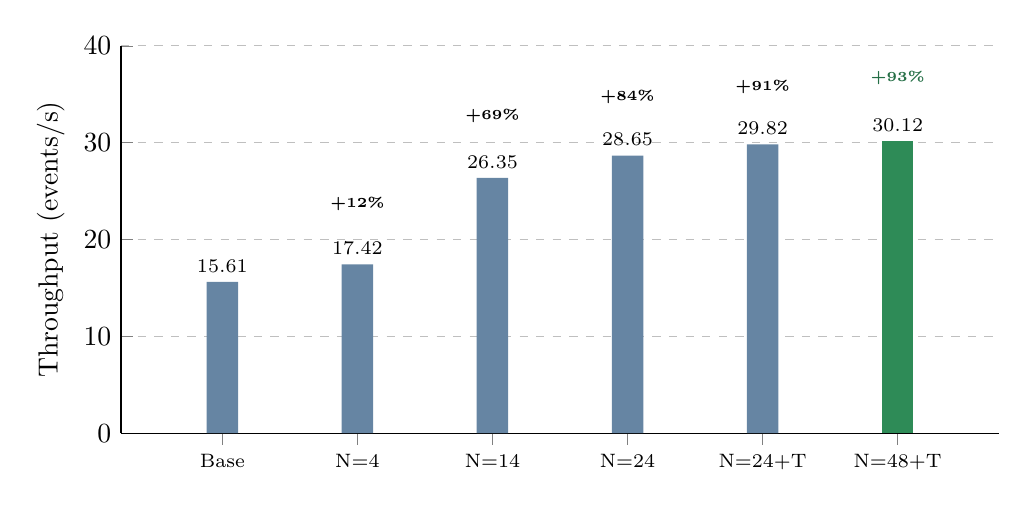
\begin{tikzpicture}
    \begin{axis}[
        ybar,
        bar shift=0pt,
        width=1.05\textwidth,
        height=6.5cm,
        ylabel={Throughput (events/s)},
        % 1. 確保符號座標包含所有點
        symbolic x coords={Base, N4, N14, N24, N24T, N48T}, 
        % 2. 將 xtick=data 改為明確列出所有座標，確保最後一項也會顯示
        xtick={Base, N4, N14, N24, N24T, N48T},
        % 3. 對應的標籤
        xticklabels={Base, N=4, N=14, N=24, N=24+T, N=48+T},
        x tick label style={font=\scriptsize, align=center},
        ymin=0, 
        ymax=40,
        bar width=0.4cm,
        enlarge x limits=0.15,
        nodes near coords,
        nodes near coords style={font=\scriptsize\bfseries},
        axis lines*=left,
        ymajorgrids=true,
        grid style=dashed,
    ]
    
    % Standard bars (藍色部分)
    \addplot[fill=acadblue!60, draw=none] coordinates {
        (Base, 15.61) 
        (N4, 17.42) 
        (N14, 26.35) 
        (N24, 28.65) 
        (N24T, 29.82)
    };
    
    % Highlighted "Optimal" bar (最右邊綠色)
    \addplot[fill=acadgreen, draw=none] coordinates {
        (N48T, 30.12)
    };
    
    % --- Annotations (百分比標籤) ---
    \node[font=\tiny\bfseries, anchor=south] at (axis cs:N4, 22) {+12\%};
    \node[font=\tiny\bfseries, anchor=south] at (axis cs:N14, 31) {+69\%};
    \node[font=\tiny\bfseries, anchor=south] at (axis cs:N24, 33) {+84\%};
    \node[font=\tiny\bfseries, anchor=south] at (axis cs:N24T, 34) {+91\%};
    \node[font=\tiny\bfseries, text=acadgreen!80!black, anchor=south] at (axis cs:N48T, 35) {+93\%};
    
    \end{axis}
\end{tikzpicture}

\column{0.35\textwidth}
% Big Result Visual
\begin{tcolorbox}[colback=green!10, colframe=acadgreen, boxrule=1.5pt, halign=center, width=\textwidth]
    \Huge \textbf{\textcolor{acadgreen}{+93\%}} \\[5pt]
    \large Throughput \\[2pt]
    \scriptsize $15.61 \rightarrow \mathbf{30.12}$ ev/s
\end{tcolorbox}

\vspace{0.5em}
\textbf{Key Milestones}
\begin{itemize}
    \item \textbf{N=14:} +69\% (batching)
    \item \textbf{N=24:} +84\% (scaling)
    \item \textbf{N=48+T:} \textcolor{acadgreen}{\textbf{+93\% (optimal)}}
\end{itemize}
\end{columns}
\end{frame}

% --- REPLACE SLIDE 11 ---
\begin{frame}{Synchronization Reduction (NSYS)}
\begin{columns}
\column{0.45\textwidth}
    % KPI Stack
    \begin{tcolorbox}[colback=green!10, colframe=acadgreen, title=Stream Synchronizations, halign=center]
        \LARGE \textbf{$\downarrow$ 92\%} \\
        \small 8,525 $\rightarrow$ 706
    \end{tcolorbox}
    
    \begin{columns}
        \column{0.5\textwidth}
        \begin{tcolorbox}[colback=gray!10, colframe=gray, halign=center, fontupper=\scriptsize]
            \textbf{$\downarrow$ 77\%}\\Kernel Launches
        \end{tcolorbox}
        \column{0.5\textwidth}
        \begin{tcolorbox}[colback=gray!10, colframe=gray, halign=center, fontupper=\scriptsize]
            \textbf{$\downarrow$ 69\%}\\Memory Ops
        \end{tcolorbox}
    \end{columns}

\column{0.55\textwidth}
\textbf{Kernel Instance Reduction (Log Scale)}
    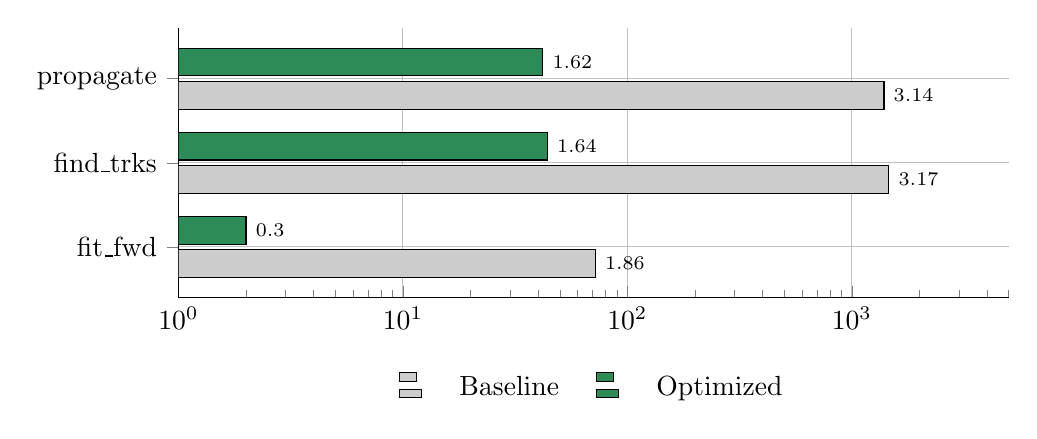
\begin{tikzpicture}
\begin{axis}[
        xbar,
        xmode=log,
        log origin=infty,
        width=\textwidth,
        height=5cm,
        log basis x=10,
        symbolic y coords={fitfwd, findtrks, propagate},
        yticklabels={fit\_fwd, find\_trks, propagate},
        ytick=data,
        point meta=rawx, 
        nodes near coords={%
            \pgfmathfloattofixed{\pgfplotspointmeta}%
            \pgfmathparse{log10(\pgfmathresult)}%
            \pgfmathprintnumber[fixed, precision=2]{\pgfmathresult}%
        },
        nodes near coords align={horizontal},
        nodes near coords style={font=\scriptsize, text=black, anchor=west},
        xmin=1,
        xmax=5000, 
        enlarge y limits=0.3,
        axis lines*=left,
        grid=major,
        % --- 修正後的 Legend Style ---
        legend style={
            at={(0.5,-0.25)}, % 確保在中間
            anchor=north, 
            legend columns=-1, 
            draw=none,
            column sep=0.4cm  % 適度的左右間隔
        }
    ]
    \addplot[fill=gray!40] coordinates {(72,fitfwd) (1463,findtrks) (1391,propagate)};
    \addplot[fill=acadgreen] coordinates {(2,fitfwd) (44,findtrks) (42,propagate)};
    \legend{Baseline, Optimized}
    \end{axis}
    \end{tikzpicture}
    
    \vspace{0.8em} % 稍微增加間距，避免 Result 擋到 Legend
    \centering
    \small \textit{Result: Same work, significantly fewer launches.}
\end{columns}
\end{frame}

\begin{frame}{Batch Size Optimization}
\begin{columns}
\column{0.58\textwidth}
\centering
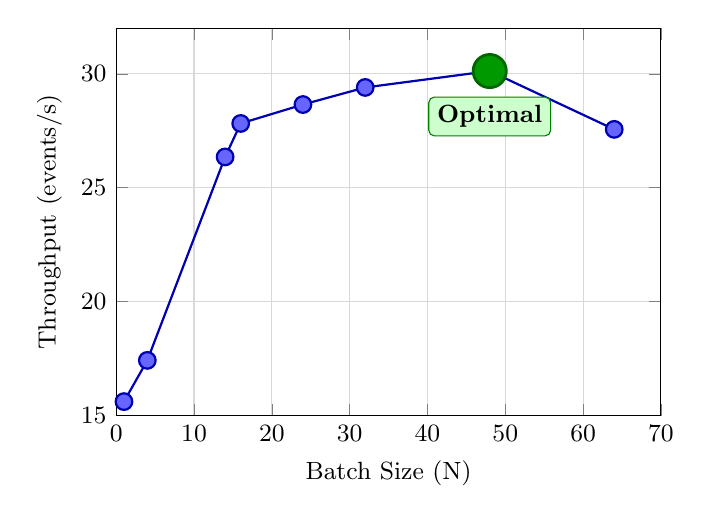
\begin{tikzpicture}[scale=1.0]
    \begin{axis}[
        width=8.5cm,
        height=6.5cm,
        xlabel={Batch Size (N)},
        ylabel={Throughput (events/s)},
        xmin=0, xmax=70,
        ymin=15, ymax=32,
        grid=major,
        grid style={gray!30},
        mark size=3pt,
        label style={font=\small},
        tick label style={font=\small},
    ]
    \addplot[blue!70!black, thick, mark=*, mark options={fill=blue!60}] coordinates {
        (1, 15.61)
        (4, 17.42)
        (14, 26.35)
        (16, 27.82)
        (24, 28.65)
        (32, 29.40)
        (48, 30.12)
        (64, 27.56)
    };
    % Prominent optimal point marker
    \addplot[only marks, mark=*, mark size=6pt, mark options={fill=green!60!black, draw=green!40!black, line width=1pt}] coordinates {(48, 30.12)};
    \node[anchor=north, fill=green!20, draw=green!50!black, rounded corners=2pt, inner sep=3pt, font=\small\bfseries] at (axis cs:48,29) {Optimal};
    \end{axis}
\end{tikzpicture}

\column{0.42\textwidth}
\textbf{Key Findings} {\small (Tesla V100-SXM2-32GB)}
\begin{itemize}
    \item Optimal batch size: \textbf{N=48}
    \item Throughput: 30.12 events/s
    \item +93\% vs no batching
\end{itemize}

\vspace{0.3em}
\begin{block}{Discovered Issues}
\begin{itemize}
    \item Memory alignment bugs at N=6,8,12
    \item OOM at N=64+ (dataset dependent)
\end{itemize}
\end{block}

\vspace{0.3em}
\textbf{Production Setting}
\begin{itemize}
    \item Default changed: 1 $\rightarrow$ 48
    \item Configurable via \texttt{--batch-size}
\end{itemize}
\end{columns}
\end{frame}

\begin{frame}{Kernel-Level Analysis (NCU)}
{\small \textit{NCU profiled on RTX 2080 Ti; throughput benchmarks on V100}}
\vspace{0.2em}
\begin{columns}
\column{0.5\textwidth}
\textbf{Occupancy Improvements}
\begin{table}
    \scriptsize
    \begin{tabular}{lccc}
        \toprule
        \textbf{Kernel} & \textbf{Base} & \textbf{Opt} & \textbf{Gain} \\
        \midrule
        fit\_forward & 15.4\% & 38.4\% & \textbf{+150\%} \\
        fit\_backward & 14.9\% & 29.9\% & \textbf{+100\%} \\
        propagate & 35.0\% & 42.8\% & +22\% \\
        find\_tracks & 21.4\% & 23.7\% & +11\% \\
        \bottomrule
    \end{tabular}
\end{table}

\vspace{0.3em}
\begin{alertblock}{Key Finding}
    Baseline fitting kernels at \textbf{15\% occupancy}---severe GPU under-utilization that batching directly addresses.
\end{alertblock}

\column{0.5\textwidth}
\textbf{Memory Throughput (GB/s)}
\begin{table}
    \scriptsize
    \begin{tabular}{lccc}
        \toprule
        \textbf{Kernel} & \textbf{Base} & \textbf{Opt} & \textbf{Gain} \\
        \midrule
        fit\_backward & 96.8 & 245.5 & \textbf{+154\%} \\
        fit\_forward & 61.5 & 135.7 & \textbf{+121\%} \\
        find\_tracks & 43.8 & 57.7 & +32\% \\
        propagate & 224.5 & 264.0 & +18\% \\
        \bottomrule
    \end{tabular}
\end{table}

\vspace{0.3em}
\textbf{Grid Size Scaling}
\begin{itemize}
    \item CKF kernels: \textbf{6.1x} larger grids
    \item Fitting kernels: \textbf{4.3x} larger grids
    \item Validates batching is working
\end{itemize}
\end{columns}
\end{frame}

\begin{frame}{Validation Results}
\begin{columns}
\column{0.5\textwidth}
% Large PASSED Badge
\centering
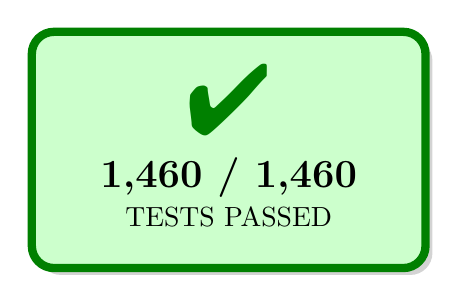
\begin{tikzpicture}
    % Main badge
    \node[draw, rounded corners=8pt, fill=green!20, minimum width=5cm, minimum height=3cm, line width=3pt, draw=green!50!black, drop shadow={shadow xshift=2.5pt, shadow yshift=-2.5pt, opacity=0.35}] at (0,0) {
        \begin{tabular}{c}
            {\fontsize{36}{40}\selectfont \textbf{\textcolor{green!50!black}{\ding{52}}}} \\[5pt]
            {\Large \textbf{1,460 / 1,460}} \\[2pt]
            {\normalsize TESTS PASSED}
        \end{tabular}
    };
\end{tikzpicture}

\vspace{0.3em}
% Test breakdown - larger font for readability
{\small
\begin{center}
\begin{tabular}{ll}
\textbf{core:} 24 & \textbf{cuda:} 710 \\
\textbf{io:} 9 & \textbf{cpu:} 714 \\
\textbf{examples:} 3 & \\
\end{tabular}
\end{center}
}

\column{0.5\textwidth}
% Validation criteria with icons
\textbf{Physics Validation}
\vspace{0.3em}

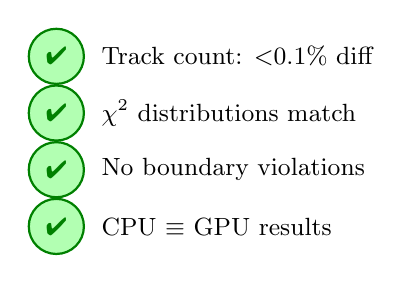
\begin{tikzpicture}[scale=0.9]
    % Track count
    \node[draw, circle, fill=green!30, minimum size=0.7cm, font=\small, line width=0.8pt, draw=green!50!black] at (0,2.4) {\textcolor{green!50!black}{\ding{52}}};
    \node[anchor=west, font=\small] at (0.5,2.4) {Track count: $<$0.1\% diff};

    % Chi-squared
    \node[draw, circle, fill=green!30, minimum size=0.7cm, font=\small, line width=0.8pt, draw=green!50!black] at (0,1.6) {\textcolor{green!50!black}{\ding{52}}};
    \node[anchor=west, font=\small] at (0.5,1.6) {$\chi^2$ distributions match};

    % Boundaries
    \node[draw, circle, fill=green!30, minimum size=0.7cm, font=\small, line width=0.8pt, draw=green!50!black] at (0,0.8) {\textcolor{green!50!black}{\ding{52}}};
    \node[anchor=west, font=\small] at (0.5,0.8) {No boundary violations};

    % CPU=GPU
    \node[draw, circle, fill=green!30, minimum size=0.7cm, font=\small, line width=0.8pt, draw=green!50!black] at (0,0) {\textcolor{green!50!black}{\ding{52}}};
    \node[anchor=west, font=\small] at (0.5,0) {CPU $\equiv$ GPU results};
\end{tikzpicture}

\vspace{0.5em}
\textbf{Stability}
\begin{itemize}
    \item 100+ events/config tested
    \item Reproducible: $<$1\% variance
\end{itemize}
\end{columns}
\end{frame}

%==============================================================================%
\section{Negative Results}
%==============================================================================%

% --- REPLACE SLIDE 15 ---
\begin{frame}{Documented Negative Results}
\centering
\textit{Scientific value: Understanding what doesn't work}

\vspace{1em}
\renewcommand{\arraystretch}{1.1} 
\setlength{\tabcolsep}{10pt}
\begin{table}
\rowcolors{2}{gray!10}{white}
\begin{tabular}{l c l}
    \toprule
    \textbf{Approach} & \textbf{Outcome} & \textbf{Lesson Learned} \\
    \midrule
    Sorting removal & \textcolor{acadred}{\ding{56}} & Sorted access improves memory coalescing \\
    Track compaction & \textcolor{acadred}{\ding{56}} & 100\% alive in early steps; +18.8\% overhead \\
    Smaller batches & \textcolor{acadred}{\ding{56}} & Insufficient parallelism for GPU saturation \\
    Persistent kernel & \textcolor{acadred}{\ding{56}} & 98\% efficiency achieved; diminishing returns \\
    Kernel fusion & \textcolor{acadred}{\ding{56}} & High register pressure reduced occupancy \\
    \bottomrule
\end{tabular}
\end{table}

\vspace{0.5em}
\begin{block}{Summary}
    Five architectural approaches were tested and rejected. These failures directly guided the successful batching strategy.
\end{block}
\end{frame}

%==============================================================================%
\section{Contributions}
%==============================================================================%

\begin{frame}{Technical Contributions}
% Infographic row of big numbers
\begin{center}
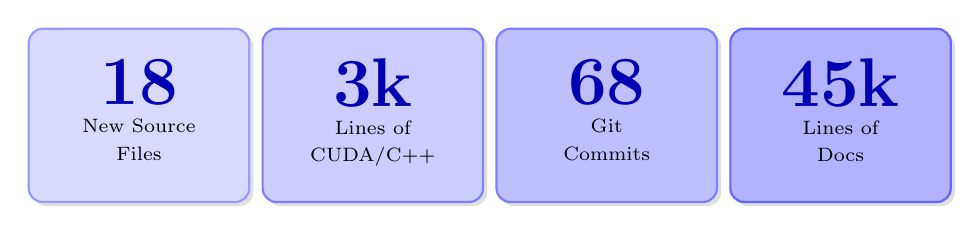
\begin{tikzpicture}[scale=0.9,
    kpibox/.style={draw, rounded corners=5pt, minimum width=2.8cm, minimum height=2.2cm, line width=0.8pt, drop shadow={shadow xshift=1.5pt, shadow yshift=-1.5pt, opacity=0.25}}]
    % New Files
    \node[kpibox, fill=blue!15, draw=blue!40] at (0,0) {
        \begin{tabular}{c}
            {\fontsize{28}{32}\selectfont \textbf{\textcolor{blue!70!black}{18}}} \\[-2pt]
            {\scriptsize New Source} \\[-2pt]
            {\scriptsize Files}
        \end{tabular}
    };

    % Lines of Code
    \node[kpibox, fill=blue!20, draw=blue!50] at (3.3,0) {
        \begin{tabular}{c}
            {\fontsize{28}{32}\selectfont \textbf{\textcolor{blue!70!black}{3k}}} \\[-2pt]
            {\scriptsize Lines of} \\[-2pt]
            {\scriptsize CUDA/C++}
        \end{tabular}
    };

    % Commits
    \node[kpibox, fill=blue!25, draw=blue!50] at (6.6,0) {
        \begin{tabular}{c}
            {\fontsize{28}{32}\selectfont \textbf{\textcolor{blue!70!black}{68}}} \\[-2pt]
            {\scriptsize Git} \\[-2pt]
            {\scriptsize Commits}
        \end{tabular}
    };

    % Documentation
    \node[kpibox, fill=blue!30, draw=blue!60] at (9.9,0) {
        \begin{tabular}{c}
            {\fontsize{28}{32}\selectfont \textbf{\textcolor{blue!70!black}{45k}}} \\[-2pt]
            {\scriptsize Lines of} \\[-2pt]
            {\scriptsize Docs}
        \end{tabular}
    };
\end{tikzpicture}
\end{center}

\vspace{0.3em}
\begin{columns}
\column{0.5\textwidth}
\textbf{Key Components}
\begin{itemize}
    \item Batched CKF wrapper ($\sim$260 lines)
    \item Constant memory infrastructure
    \item Device-side concatenation kernels
    \item Inline Thrust replacements
\end{itemize}

\column{0.5\textwidth}
\textbf{Documentation}
\begin{itemize}
    \item $\sim$100 markdown documents
    \item Optimization plans \& analysis
    \item Safety proofs (sync removal)
    \item Negative results documentation
\end{itemize}
\end{columns}
\end{frame}

%==============================================================================%
\section{Conclusion}
%==============================================================================%

\begin{frame}{Summary and Future Work}
\begin{columns}
\column{0.5\textwidth}
\textbf{Achievements}
\begin{itemize}
    \item +93\% throughput improvement
    \item 1,460/1,460 tests passing
    \item Production-ready implementation
    \item Exceeded 50\% target
\end{itemize}

\vspace{0.3em}
\textbf{Key Innovations}
\begin{itemize}
    \item Multi-event batching with event isolation
    \item Device-side concatenation (D2D vs D-H-D)
    \item Constant memory + stream-ordered execution
    \item \textbf{98\% of theoretical efficiency achieved}
\end{itemize}

\column{0.5\textwidth}
\textbf{Future Work}
\begin{itemize}
    \item Multi-GPU scaling investigation
    \item CPU-GPU pipelining (analyzed: +2\% headroom)
    \item Memory alignment bug fix (N=6,8,12)
    \item Upstream contribution to ACTS
\end{itemize}

\vspace{0.3em}
\textbf{Timeline}
\begin{itemize}
    \item Nov 15 - Dec 21, 2025: Implementation
\end{itemize}
\end{columns}

\vspace{0.3em}
\begin{block}{Conclusion}
    Achieved \textbf{+93\% throughput improvement} in GPU track reconstruction, exceeding the 50\% target while maintaining full correctness.
\end{block}
\end{frame}

\begin{frame}{Questions?}
\begin{center}
\vspace{1em}

% Key result reminder
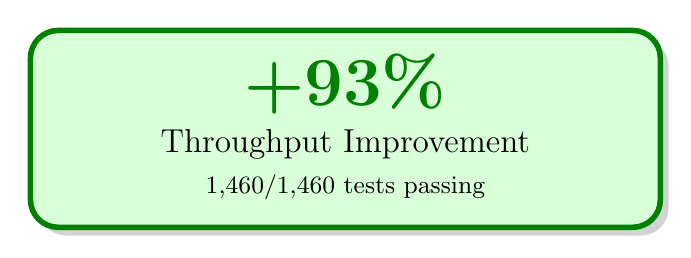
\begin{tikzpicture}
    \node[draw, rounded corners=10pt, fill=green!15, minimum width=8cm, minimum height=2.5cm, line width=2pt, draw=green!50!black, drop shadow={shadow xshift=3pt, shadow yshift=-3pt, opacity=0.35}] at (0,0) {
        \begin{tabular}{c}
            {\Huge \textbf{\textcolor{green!50!black}{+93\%}}} \\[5pt]
            {\large Throughput Improvement} \\[3pt]
            {\small 1,460/1,460 tests passing}
        \end{tabular}
    };
\end{tikzpicture}

\vspace{1.5em}
{\Large Thank you for your attention!}

\vspace{1.5em}
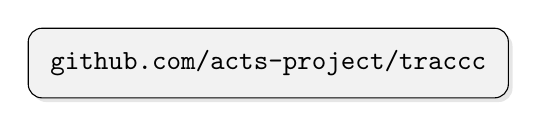
\begin{tikzpicture}
    \node[draw, rounded corners=5pt, fill=gray!10, inner sep=8pt, drop shadow={shadow xshift=1.5pt, shadow yshift=-1.5pt, opacity=0.2}] {
        \texttt{github.com/acts-project/traccc}
    };
\end{tikzpicture}
\end{center}
\end{frame}

%==============================================================================%
% BACKUP SLIDES
%==============================================================================%
\appendix

\begin{frame}{Backup: Anticipated Questions (1/6)}
\textbf{Q1: Why is batch size 48 optimal? Why not higher?}
\begin{itemize}
    \item At N=48, we hit V100 memory bandwidth ceiling
    \item N=64 causes memory pressure and cache thrashing
    \item Pre-existing alignment bugs at N=6,8,12 constrain options
\end{itemize}

\vspace{0.5em}
\textbf{Q2: How do you ensure tracks don't cross event boundaries?}
\begin{itemize}
    \item \texttt{get\_event\_id()} called for every candidate-measurement link
    \item Binary search in O(log N) with constant memory = near-zero overhead
    \item Reject links where seed and measurement have different event IDs
\end{itemize}

\vspace{0.5em}
\textbf{Q3: Why did track compaction fail?}
\begin{itemize}
    \item In early CKF steps (1-4), 100\% of candidates still alive
    \item Compaction overhead: buffer allocation, kernel launch, sync
    \item Would need selective compaction only for later steps
\end{itemize}
\end{frame}

\begin{frame}{Backup: Anticipated Questions (2/6)}
\textbf{Q4: How confident are you in correctness?}
\begin{itemize}
    \item 1,460 automated tests (unit + physics validation)
    \item GPU vs CPU reference: $<$0.1\% track count tolerance
    \item Extensive manual validation on ttbar\_mu200 dataset
\end{itemize}

\vspace{0.5em}
\textbf{Q5: What's the theoretical maximum speedup?}
\begin{itemize}
    \item CKF is memory-bound with $\sim$42\% DRAM utilization
    \item Theoretical max with perfect coalescing: $\sim$2.5x current
    \item Scattered access pattern is fundamental to algorithm
    \item 93\% captures most ``easy'' gains; further needs algorithmic changes
\end{itemize}

\vspace{0.5em}
\textbf{Q6: Can this work apply to other traccc algorithms?}
\begin{itemize}
    \item Yes: \texttt{batch\_metadata} and concatenation kernels are generic
    \item Constant/texture memory patterns also reusable
    \item Code designed to be modular for seeding/fitting
\end{itemize}
\end{frame}

\begin{frame}{Backup: Anticipated Questions (3/6)}
\textbf{Q7: What was most challenging?}
\begin{itemize}
    \item Chi-squared bug: GPU produced ``reasonable'' but wrong results
    \item Required line-by-line comparison of GPU vs CPU code paths
    \item Lesson: exact CPU reference implementations are essential
\end{itemize}

\vspace{0.5em}
\textbf{Q8: How long did this take?}
\begin{itemize}
    \item Main implementation: 5--6 weeks (Nov 15 -- Dec 21, 2025)
    \item Significant time spent on failed approaches that guided success
\end{itemize}

\vspace{0.5em}
\textbf{Q9: How was sync removal proven safe?}
\begin{itemize}
    \item \texttt{par\_nosync} policy guarantees stream-ordered execution
    \item CUDA semantics: operations in same stream execute in order
    \item Documented safety proofs in $\sim$45,000 lines of analysis
\end{itemize}
\end{frame}

\begin{frame}{Backup: Anticipated Questions (4/6)}
\textbf{Q10: What about the vecmem memory alignment bugs?}
\begin{itemize}
    \item Pre-existing bugs in vecmem library, not caused by our changes
    \item Triggered at specific batch sizes (N=6, 8, 12)
    \item Future work: investigate and fix upstream
    \item Workaround: avoid those batch sizes in production
\end{itemize}
\end{frame}

\begin{frame}{Backup: Anticipated Questions (5/6)}
\textbf{Q11: How did you validate at kernel level?}
\begin{itemize}
    \item Used NVIDIA Nsight Compute (NCU) for per-kernel metrics
    \item Compared occupancy, memory throughput, cache hit rates
    \item Confirmed baseline fitting kernels at 15\% occupancy (85\% idle)
\end{itemize}

\vspace{0.4em}
\textbf{Q12: Why do cache hit rates decrease but performance improves?}
\begin{itemize}
    \item Batching increases working set size $\rightarrow$ lower L1 hit rate (48\%$\rightarrow$43\%)
    \item But better memory coalescing $\rightarrow$ +154\% throughput
    \item Trade-off: bandwidth utilization beats cache efficiency
\end{itemize}

\vspace{0.4em}
\textbf{Q13: What does NCU reveal about future opportunities?}
\begin{itemize}
    \item fit\_forward at 38\%, fit\_backward at 30\% occupancy---headroom remains
    \item Kernels are memory-bound with scattered access patterns
    \item Further gains require algorithmic changes to improve locality
\end{itemize}
\end{frame}

\begin{frame}{Backup: NCU Profiling Details (6/6)}
{\small \textbf{Hardware:} NVIDIA GeForce RTX 2080 Ti (CC 7.5, 68 SMs)}

\vspace{0.2em}
\begin{columns}
\column{0.55\textwidth}
\textbf{Per-Kernel Metrics}
\vspace{-0.3em}
\begin{table}
    \scriptsize
    \setlength{\tabcolsep}{3pt}
    \begin{tabular}{lccc}
        \toprule
        \textbf{Kernel} & \textbf{Occ.} & \textbf{Mem} & \textbf{Grid} \\
        \midrule
        \multicolumn{4}{l}{\textit{Baseline}} \\
        propagate & 35.0\% & 224 GB/s & 236 \\
        find\_tracks & 21.4\% & 43.8 GB/s & 471 \\
        fit\_forward & 15.4\% & 61.5 GB/s & 112 \\
        fit\_backward & 14.9\% & 96.8 GB/s & 112 \\
        \midrule
        \multicolumn{4}{l}{\textit{Optimized (batch-48)}} \\
        propagate & 42.8\% & 264 GB/s & 1435 \\
        find\_tracks & 23.7\% & 57.7 GB/s & 2870 \\
        fit\_forward & 38.4\% & 135.7 GB/s & 482 \\
        fit\_backward & 29.9\% & 245.5 GB/s & 482 \\
        \bottomrule
    \end{tabular}
\end{table}

\column{0.45\textwidth}
\textbf{Cache Performance}
\vspace{-0.3em}
\begin{table}
    \scriptsize
    \begin{tabular}{lccc}
        \toprule
        \textbf{Metric} & \textbf{Base} & \textbf{Opt} & \textbf{$\Delta$} \\
        \midrule
        L1 Hit Rate & 48\% & 43\% & -11\% \\
        L2 Hit Rate & 78\% & 77\% & -2\% \\
        \bottomrule
    \end{tabular}
\end{table}

\vspace{0.2em}
\begin{alertblock}{Trade-off Analysis}
\small
Cache hit rates decrease due to larger working sets, offset by:
\begin{itemize}
    \setlength{\itemsep}{0pt}
    \item Better memory coalescing
    \item Higher bandwidth utilization
    \item \textbf{+154\%} memory throughput
\end{itemize}
\end{alertblock}
\end{columns}
\end{frame}

\end{document}
